\documentclass[11pt,a4paper]{article}
\usepackage[margin=1in]{geometry}
\usepackage{amsmath,amssymb,amsthm}
\usepackage{xcolor}
\usepackage{booktabs}
\usepackage{longtable}
\usepackage{enumitem}
\IfFileExists{titlesec.sty}{%
  \usepackage{titlesec}%
  \titleformat{\section}{\large\bfseries\color{harborblue}}{\thesection}{0.7em}{}%
  \titleformat{\subsection}{\normalsize\bfseries}{\thesubsection}{0.6em}{}%
}{}
\usepackage[colorlinks=true,linkcolor=blue!45!black,urlcolor=blue!45!black]{hyperref}
\usepackage{tikz}
\IfFileExists{pgfplots.sty}{%
  \usepackage{pgfplots}%
  \pgfplotsset{compat=1.18}%
}{}
\usetikzlibrary{arrows.meta,positioning,fit,backgrounds,calc,shapes.geometric,shapes.symbols,decorations.pathmorphing,decorations.pathreplacing}
\definecolor{harborblue}{RGB}{30,70,110}
\definecolor{shipred}{RGB}{140,30,30}
\definecolor{seagreen}{RGB}{31,110,70}
\definecolor{slate}{RGB}{71,85,105}
\definecolor{slatedark}{RGB}{30,41,59}
\definecolor{amber}{RGB}{217,119,6}
\definecolor{emerald}{RGB}{16,185,129}
\newtheorem{theorem}{Theorem}
\newtheorem{claim}{Claim}
\theoremstyle{definition}
\newtheorem{change}{Change}
\newtheorem{move}{Move}
\theoremstyle{remark}
\newtheorem*{verdict}{Verdict}
\newtheorem*{adj}{Adjudication}
\setlist{itemsep=1pt,topsep=2pt}

% Shared native-figure styles for the harbor-research corpus (relation-maps,
% regime diagrams, and data plots). Vector TikZ/pgfplots only -- see
% docs/harbor-research/figures/CONVENTION.md for the house rule this follows.
\tikzset{
  relnode/.style={draw,rounded corners,thick,minimum width=2.6cm,minimum height=0.9cm,align=center,font=\small},
  relarrow/.style={-{Stealth[length=2.5mm]},thick},
  regimebox/.style={draw,thick,align=center,font=\small,inner sep=4pt},
}
\IfFileExists{pgfplots.sty}{%
\pgfplotsset{
  harbor curve/.style={
    width=0.46\textwidth,height=5.6cm,
    axis lines=left,
    label style={font=\scriptsize},
    tick label style={font=\scriptsize},
    title style={font=\small,align=center,yshift=2pt},
    legend style={font=\scriptsize,draw=black!25,fill=white,fill opacity=0.92,text opacity=1,rounded corners=1pt,inner sep=3pt},
    thick,
  },
  harbor bar/.style={
    width=0.46\textwidth,height=5.6cm,
    ybar,bar width=6pt,
    ymode=log,log origin=infty,
    axis lines=left,
    label style={font=\scriptsize},
    tick label style={font=\tiny},
    xticklabel style={rotate=40,anchor=east,font=\tiny,inner sep=1pt},
    title style={font=\small,align=center,yshift=2pt},
    legend style={font=\scriptsize,draw=black!25,fill=white,fill opacity=0.92,text opacity=1,rounded corners=1pt,inner sep=3pt},
  },
}
}{}

\usepackage{graphicx}
\graphicspath{{../figures/}}
\usepackage{mdframed}
\newmdenv[backgroundcolor=blue!4,linecolor=harborblue,linewidth=0.8pt,skipabove=6pt,skipbelow=6pt]{thebox}
\newmdenv[backgroundcolor=red!4,linecolor=shipred,linewidth=0.8pt,skipabove=6pt,skipbelow=6pt]{boundary}
\newcommand{\onebreath}[1]{\begin{center}\emph{#1}\end{center}}

\title{\textbf{The Sealed Harbor}\\[4pt]
\large Mutually Confidential Computation with Explicit, Gated, Bounded Releases\\[3pt]
\normalsize Paper 4 of the Harbor program --- the four-pillar assurance argument, executed}
\author{Prepared for Erich Owens}
\date{August 2026}
\begin{document}
\maketitle

\begin{abstract}
\noindent Two parties who will share neither data nor model can nonetheless obtain an attributable, policy-bound joint
computation, with every information release explicit, gated, and bounded --- and the security boundary is the declassification
gate, not token-level taint. We present the clean-room design for tool-using LLM agents (dual-attested key release, whole-worker
taint, two declassification gates) and its assurance argument as four independently verified pillars: (1) observational
noninterference modulo declassification, verified exhaustively on the finite clean-room model with a mutation suite that catches
both canonical breaks; (2) the supervisory-control result that fixes \emph{which} boundary can be enforced at all --- the channel,
never the token; (3) $\varepsilon$-conservation of the release ledger, with differential-privacy composition giving the conserved
sum its meaning; and (4) a canary detection theory with a quotable operating curve and a sequential-test alarm clock. We price the
residual honestly: an information-theoretic leakage budget of $q\cdot b$ bits across $q$ jobs through any $b$-bit release channel,
before timing channels, which are out of model. \emph{Express lane: the one-breath claim of each pillar opens its section; the
formal statement is in the box below it; a reader in a hurry needs nothing else.}
\end{abstract}

\section{The problem: Derek and Erin}\label{sec:problem}

\textbf{The scene.} Derek owns sensitive financial data $D$. Erin owns a valuable agent system $M$ --- weights, prompts, skills,
tools, orchestration. Both want the answer $y=f_M(D)$. Neither will hand over the crown jewels: Derek must not receive $M$, Erin
must not receive $D$, and the cloud operator hosting the computation must receive neither. Every week some enterprise negotiates
this exact standoff with lawyers and air-gapped laptops; the question is whether a \emph{computational} contract can replace the
lawyers' one --- and what, precisely, it can promise.

The tempting pitch --- and the one an early product review of this program actually wrote --- is a ``silicon-enforced NDA'': tag
Erin's agent \texttt{[TAINT:HIGH]} the moment it reads Derek's data, drop any tainted egress packet, and declare that the data
``mathematically cannot phone home.'' This paper's first job is to explain why that sentence must never be shipped, and its second
job is to prove the sentence that replaces it. Token-level taint through an LLM is not soundly definable: the model taints
everything it writes with everything it read, so a taint tracker faces a binary choice between marking every output token
(useless) and missing semantic flows (unsound). A secret can ride out in wording, punctuation, error messages, output length, or
timing; no regex, PII scanner, or second LLM can certify that arbitrary prose contains no secret. And an ordinary remote model API
is \emph{itself} a trusted reader of plaintext --- cryptography cannot repair sending Derek's data to a third party's inference
endpoint.

The honest architecture therefore controls the \emph{channel}, not the token, and \S\ref{sec:design} lays it out. The design
converts the question a CISO will actually ask --- \emph{how do I know the wall has no other holes?} --- into four provable
claims, one per section below: the gate is the only hole (\S\ref{sec:p1}); the gate sits on the only boundary that can be enforced
at all (\S\ref{sec:p2}); what passes through it is metered by a conserved budget (\S\ref{sec:p3}); and what tries to sneak around
the meter is caught with quotable probability and latency (\S\ref{sec:p4}). Section \ref{sec:budget} composes the pillars into a
single leakage account, and \S\ref{sec:cannot} states, at equal prominence, what none of this promises.

Each pillar section opens with its idea in one breath --- an italic express-lane sentence an expert can read alone before jumping
to the formal box --- and closes with an honest-boundary block at the same prominence as the claim. Every number carries a
provenance tag: [verified] means externally recomputable (a textbook value or a closed form restated in the box); [internal,
\emph{script}] means it regenerates from the named self-contained script at seed 20260816, shipped with the paper.

\section{The design: one work order, two fences, two gates}\label{sec:design}

\textbf{The work order.} Both principals sign the same contract before any key is released:
\[
\begin{aligned}
C=\bigl\langle\, & H(\text{data manifest}),\,H(\text{agent
bundle}),\,H(\text{runtime}),\,H(\text{policy}),\,
\text{function},\,\text{tools},\\
& \text{recipients},\,\text{output
schemas},\,\text{budgets},\,\text{retention},\,\text{validators},\,\text{payment},\,\text{liability}\,\bigr\rangle.
\end{aligned}
\]
The order names the measured runtime and agent bundle, the encrypted data inputs, the allowed tools and external providers, the
result and telemetry schemas, the output-bit/query/timing budgets, the declassification authorities, retention and key
destruction, success evidence, dispute procedure, and guarantee. Any change makes a new hash and requires both signatures.

\textbf{Dual-attested key release.} The workload boots in a confidential VM and creates an ephemeral job key with fresh
attestation evidence binding runtime, policy, worker image, key, nonce, and epoch. Derek and Erin \emph{independently} verify the
attestation; Derek's key broker releases the data key only to the approved measurement, and Erin's key broker releases the
model/skill key under the same condition --- the attester/verifier/relying-party pattern of IETF RATS \cite{rats}. The job then
runs with no ambient network or credentials. Neither principal, and not the cloud operator, can read the other's plaintext: the
room is sealed from three sides at once.

\textbf{Two fences.} Erin's worker is treated as hostile even if Erin is honest --- prompt injection or a compromised dependency
can turn a loyal agent into an exfiltrator --- so it receives \emph{semantic handles only}:
$\mathtt{read}(\text{handle},\text{range})$, $\mathtt{infer}(\text{model handle},\text{prompt handle})$,
$\mathtt{execute}(\text{tool handle},\text{args})$, $\mathtt{write}(\text{result handle},\text{bytes})$,
$\mathtt{request\_declassification}(\text{candidate handle},\text{channel})$. An attested in-guest monitor mediates labels,
handles, and encrypted content; a Derek-controlled outer gateway mediates network, storage, timing, destination, and volume.
Direct outbound TLS is forbidden; permitted services terminate at a policy gateway. And because an ordinary remote model API is
itself a trusted reader of plaintext, the model runs \emph{inside} the confidential domain --- an external inference endpoint
would be a third principal the contract never admitted.

\textbf{Whole-worker taint and two gates.} After the first secret read the entire worker state, and every later emission, is
conservatively tainted until job destruction --- decentralized labels in the Myers--Liskov style \cite{myers-liskov}, owned by
mutually distrustful principals, under which ordinary computation can only \emph{add} restrictions. Removing an owner's clause
requires a declassification authority delegated by that owner, and the only exits are the two declassification gates --- Derek's
and Erin's, each executing a declared release function --- with exactly three pre-authorized channels: a rich result to
Derek; fixed-schema, aggregated or differentially private feedback to Erin; a padded public receipt to both. Each party gets an
audience-redacted signed receipt $R=\mathrm{Sign}\bigl(H(C),H(\text{attestation}),H(\text{inputs}),H(M),H(\text{output
ciphertext}),\text{labels},\text{declassifications},\text{counters},\text{nonce},\text{epoch}\bigr)$, Merkle-anchored in both
principals' ledgers. The receipt proves what the measured system reported under a policy; it does not prove the answer is true,
nor that no unmodeled side channel existed.

Alongside the four pillars, the design carries a set of deliberately tractable side properties --- label monotonicity (no label
weakens without a declassification witness), complete mediation (every release has exactly one gate decision), provenance closure
(every release traces to committed input, model, runtime, policy, and declassifier nodes), replay safety (each job nonce settles
at most once), measurement binding (neither secret key is released for a different runtime or policy), and rollback detectability
(accepted epochs strictly increase in both external ledgers). These are design invariants backed by implementation and tests, not
theorems; the program's discipline is to label every important statement as theorem, design invariant, model-checked property, or
empirical hypothesis, and never let one impersonate another.

\begin{center}
\begin{tabular}{@{}llll@{}}
\toprule
Pillar & Claim & Verification & Artifact \\
\midrule
I (\S\ref{sec:p1}) & NI modulo declassification & exhaustive, depth 7; 2/2 mutations &
\texttt{c1\_noninterference.py} \\
II (\S\ref{sec:p2}) & enforceable $=$ controllable & product-automaton checker &
\texttt{b3\_controllability.py} \\
III (\S\ref{sec:p3}) & $\varepsilon$-ledger conserves & exhaustive $+$ 2000 random; 2/2 mut. &
\texttt{a3\_epsilon\_ledger.py} \\
IV (\S\ref{sec:p4}) & canary power $+$ SPRT clock & analytic vs.\ simulation agreement &
\texttt{a4\_canary\_sprt.py} \\
\bottomrule
\end{tabular}
\end{center}

The four rows are not four independent guarantees stacked for redundancy; they are four links in one pipeline, each closing a gap
the others leave open, in exactly the order Figure~\ref{fig:pillars} draws it. Enforceability (II) fixes \emph{where} a boundary
can exist at all --- gate the channel, or nothing about the design is provably enforceable. Noninterference (I) then proves that
boundary, once installed, is silent except through its declared release. Conservation (III) meters the cumulative cost of
everything that legitimately crosses it, because a gate honest on every single release can still bankrupt the contract over many
releases --- an individually-sound decision rule is not a portfolio-sound one. And detection (IV) polices for what tries to cross
without going through the meter at all: a compromised worker, a bug, an adversary who found an unmediated path. Drop any one link
and a concrete gap reopens, named inside its box in the figure below; the composed result --- an honestly bounded leakage account,
not an eliminated one --- is \S\ref{sec:budget}.

\begin{figure}[htbp]
\centering
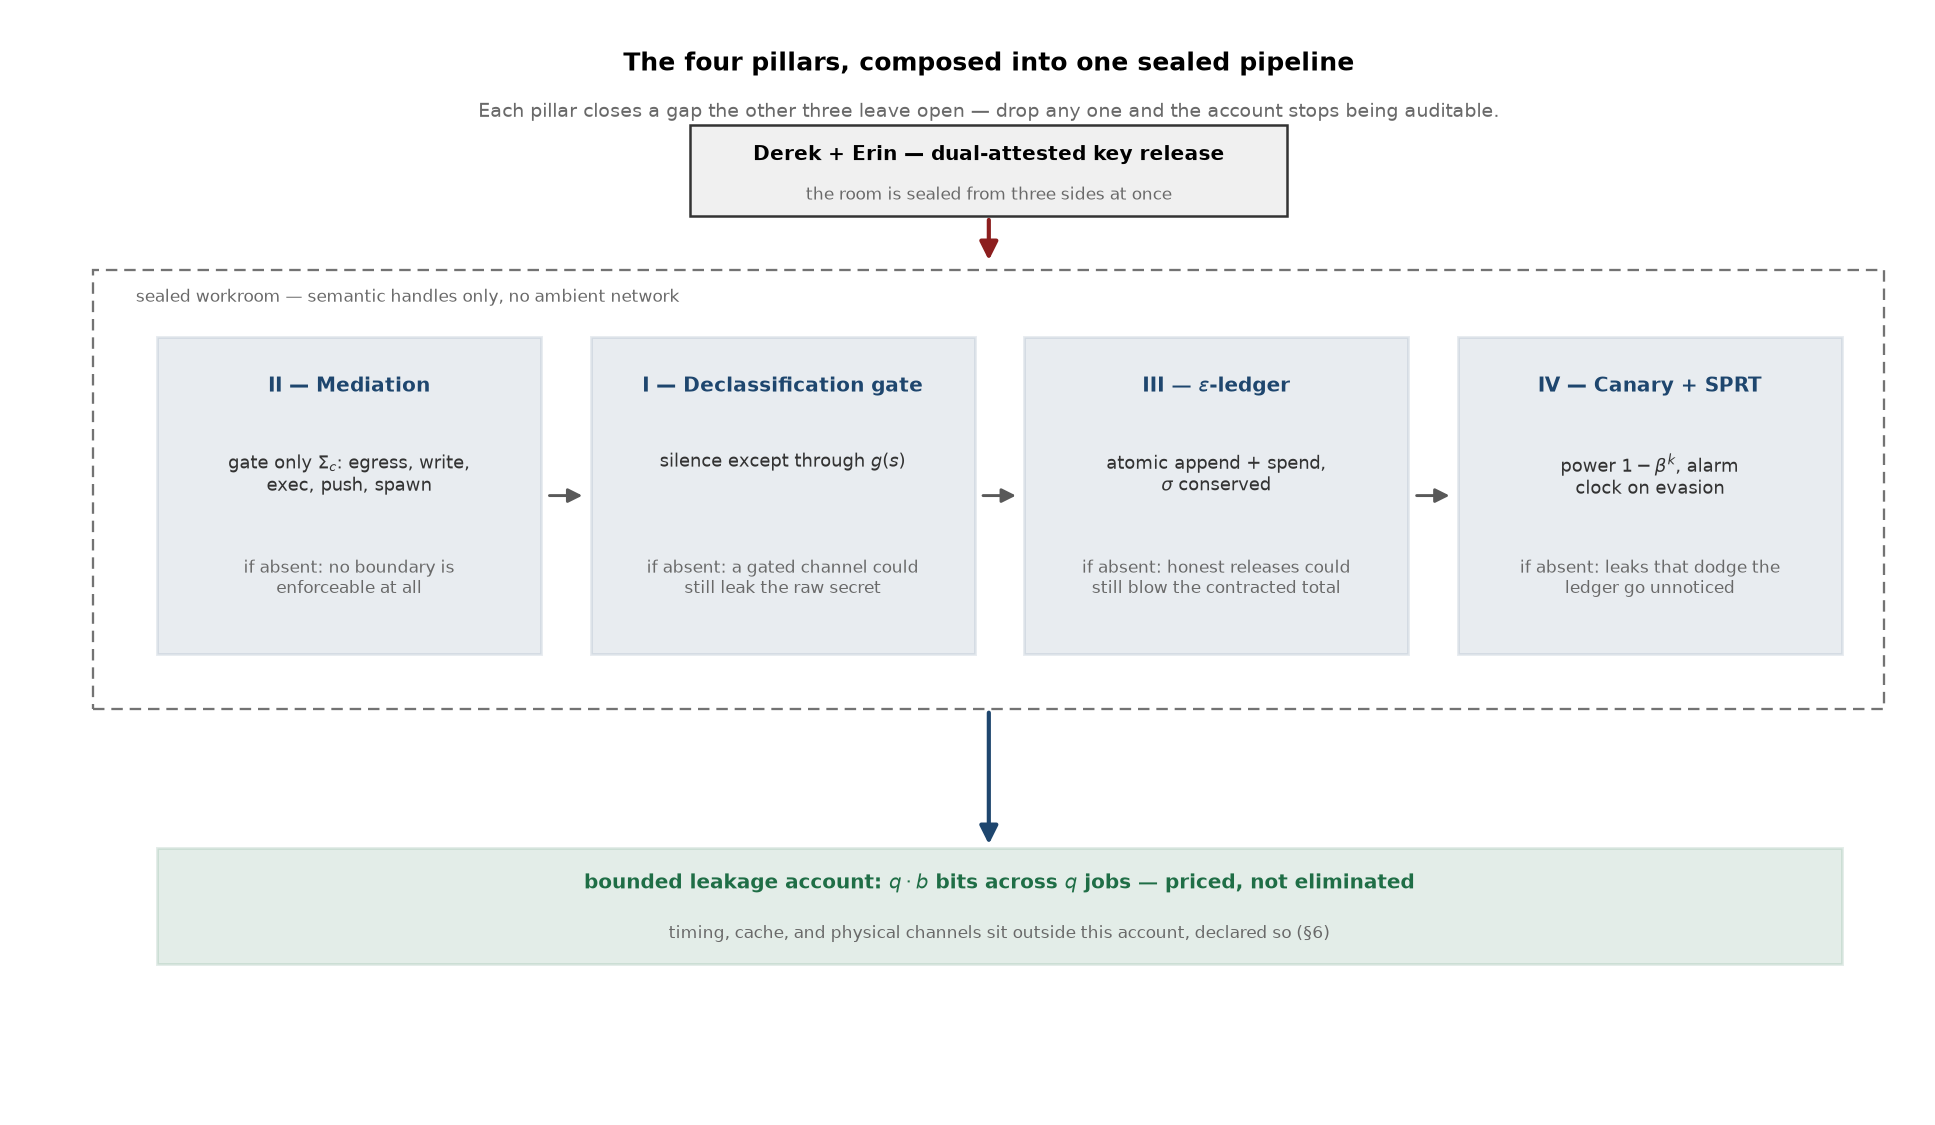
\includegraphics[width=0.95\textwidth]{paper4_pillars_architecture.png}
\caption{The four pillars composed into the sealed pipeline, in the order the closing section states it: enforceability (II) says
where the boundary can be, noninterference (I) says the boundary holds, conservation (III) meters what crosses it, detection (IV)
polices evasion. Each box also names the gap left open if that pillar alone were dropped.}
\label{fig:pillars}
\end{figure}

\section{Pillar I: silence except through the slot}\label{sec:p1}

\onebreath{Run the whole world twice --- identical except for Derek's secret --- under every
possible sequence of moves, and prove Erin's view is bit-for-bit identical whenever the gate's declared function maps the two
secrets to the same release --- formal statement in the box below.}

\textbf{Intuition.} You cannot inspect a wall for holes by staring at bricks; you inspect it by standing outside in two parallel
worlds and asking whether anything you can see ever differs. If Derek's secret is $0$ in one world and $2$ in the other, and the
gate is contracted to release only \emph{parity}, then a sound room makes those worlds indistinguishable to Erin forever, under
every interleaving of loads, reads, submissions, releases, and reports. The analogy with teeth is the voting booth: the turnstile
clicks once per voter and the tally board shows only party totals; a poll-watcher outside learns exactly the declared aggregate
and nothing about any ballot, \emph{no matter how long she watches or in what order voters arrive}. That is noninterference
\emph{modulo declassification} in the Goguen--Meseguer lineage \cite{goguen-meseguer-82,goguen-meseguer-84}: silence except
through the slot, and through the slot, only what the contract says. Figure~\ref{fig:r9rel} draws the mapping by relations, not
surface features. The misread to preempt: the theorem does not say the slot is safe --- it says the slot is the \emph{only}
opening; whether the declared function $g$ releases too much is a contract question the next two pillars price.

\begin{figure}[htbp]
\centering
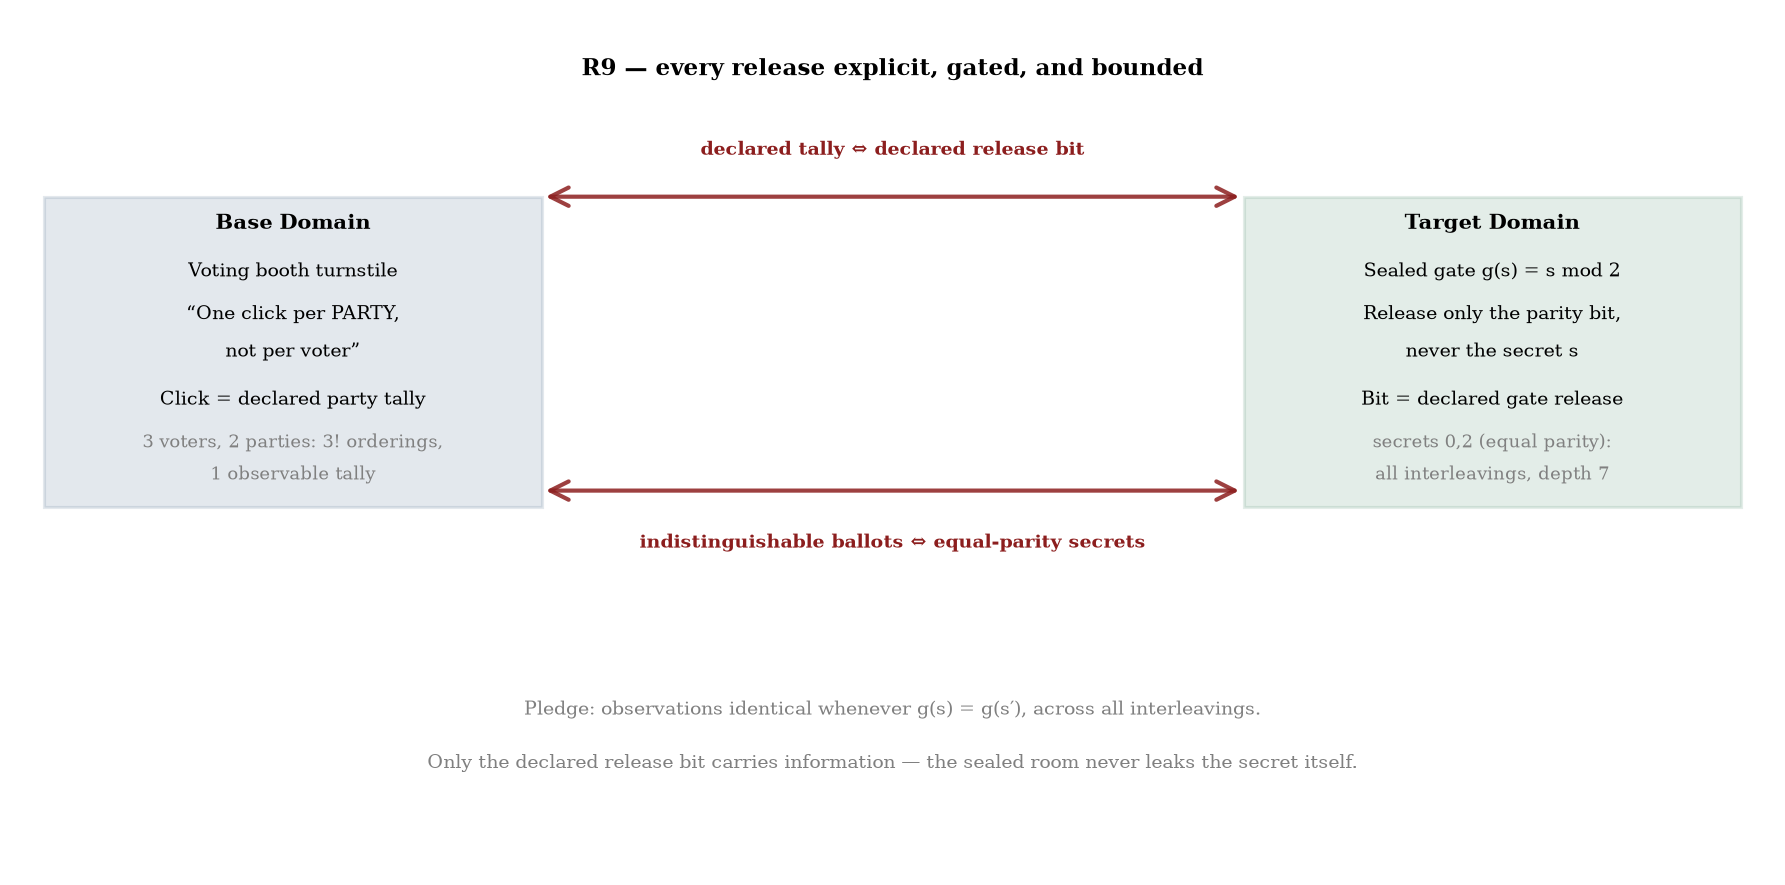
\includegraphics[width=0.92\textwidth]{r9_relation.png}
\caption{Relation-map for Pillar I. The voting booth maps to the sealed workroom by
\emph{relations}, not surface features: booth walls $\to$ attested isolation (no observation of the work); the tally board $\to$
the declassification gate (the sole declared release); ``watching all day reveals no ballot'' $\to$ two-run observational
equivalence under every interleaving. The analogy predicts, correctly, that the residual risk is a too-revealing tally --- a
per-precinct board with one voter is a leaky $g$.}
\label{fig:r9rel}
\end{figure}

\begin{thebox}
\textbf{Theorem 1 (noninterference modulo declassification; finite model, exhaustive).} Fix the clean-room transition system with
secrets $s\in\{0,1,2,3\}$, Erin-observable state $\mathrm{Obs}_E$, and declared release function $g(s)=s\bmod 2$. For secrets
$s,s'$ and \emph{every} action sequence: if $g(s)=g(s')$ then Erin's observation sequences are identical; if $g(s)\neq g(s')$ they
may differ only at explicit gate-release steps.

\textbf{Verification.} Exhaustive over all interleavings to depth 7 $\times$ all secret pairs: zero distinguishing observations in
the honest model [internal, \texttt{c1\_noninterference.py}]. The schedule itself is secret-independent, checked separately --- an
enabledness difference would itself be a channel. The Rushby unwinding condition \emph{local respect} (Derek-side actions never
touch Erin-observable state) holds mechanically \cite{rushby}. \textbf{Mutations:} (m1) a gate that leaks the raw secret is caught
distinguishing secrets $(0,2)$ --- an \emph{equal-parity} pair the honest gate provably keeps identical --- with witness trace
$\mathtt{load}\to\mathtt{read}\to\mathtt{submit}\to\mathtt{release}$, after which Erin sees \texttt{(gate,0)} in one world and
\texttt{(gate,2)} in the other; (m2) a worker bypassing the gate is caught in a 3-step trace. Reverting the mutations restores the
property [internal, \texttt{c1\_noninterference.py}].
\end{thebox}

\textbf{Numbers by hand.} Four secrets give $\binom{4}{2}=6$ unordered pairs; two of them --- $(0,2)$ and $(1,3)$ --- are
equal-parity, and it is exactly those two on which the honest gate must keep Erin's worlds identical forever, and did. The m1
witness is a four-step, human-readable proof that a particular gate breaks its contract; a CISO can read it aloud. The full mutant
grid, honest gate against both breaks, is Figure~\ref{fig:r9reg}.
\emph{Now you try:} with $g(s)=s\bmod 2$ over secrets $\{0,\dots,7\}$, how many unordered secret pairs must a sound room keep
Erin-indistinguishable? (Both parity classes have four members: $2\binom{4}{2}=12$ pairs.)

\textbf{What it buys.} The product's headline sentence in its corrected, provable form: \emph{every release is explicit, gated,
and bounded}. This is the finite-model core of the paper; the general theorem over unbounded state is the Isabelle/AFP unwinding
obligation (\S\ref{sec:lift}), for which this model is the blueprint --- the same three unwinding conditions, discharged
mechanically rather than exhaustively.

\begin{boundary}
\textbf{Honest boundary.} Finite depth, finite secrets: depth-7 exhaustion is a proof about the model, not the deployment; the
lift is \S\ref{sec:lift}'s job. The guarantee is possibilistic --- timing, token counts, and termination channels are out of
model, as the design declares (\S\ref{sec:cannot}). The gate's \emph{specification} is the residual oracle: we prove releases
match $g$; choosing a $g$ that leaks too much is a contract failure no theorem prevents --- that risk is priced, not eliminated,
by Pillars III--IV. And a human who reads a released parity may still remember it: the system bounds channels, not minds.
\end{boundary}

\begin{figure}[htbp]
\centering
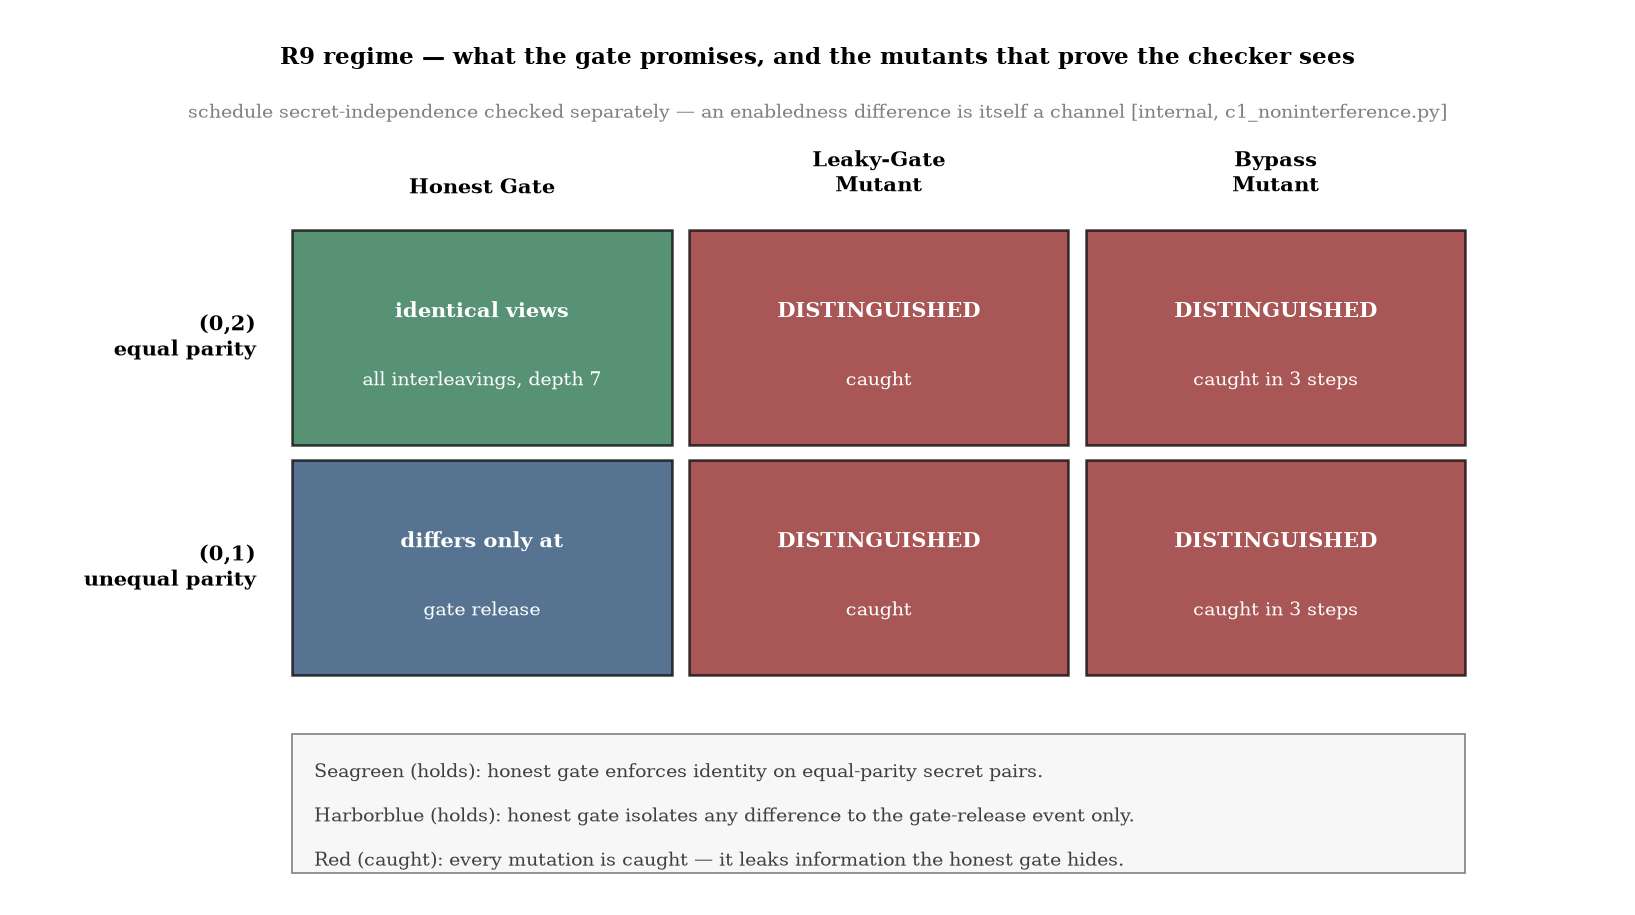
\includegraphics[width=0.92\textwidth]{r9_regime.png}
\caption{Regime diagram for Pillar I: what the gate promises, and the mutants that prove the checker
sees. The property holds on the shaded region (equal declassified value, any interleaving); the two mutation witnesses (leaky
gate; gate bypass) sit provably outside it, each with a concrete trace
[internal, \texttt{c1\_noninterference.py}].}
\label{fig:r9reg}
\end{figure}

\section{Pillar II: the channel, never the token}\label{sec:p2}

\onebreath{A safety policy over an agent's behavior can be enforced by a hypervisor if and only if
it constrains only events the hypervisor mediates --- so the enforceable clean-room boundary is the egress channel, and any
promise phrased over model-internal events is detect-only forever --- formal statement in the box below.}

\textbf{Intuition.} A bouncer at the door of a club can prevent anyone from \emph{entering or leaving}; no bouncer can prevent a
patron from \emph{thinking about} leaving. Split the agent's event alphabet accordingly: controllable events the mediation layer
can veto ($\Sigma_c$: \texttt{fs\_write}, \texttt{net\_egress}, \texttt{exec\_tool}, \texttt{git\_push}, \texttt{spawn\_child})
and uncontrollable events it can at best observe ($\Sigma_u$: \texttt{model\_emit\_token}, \texttt{in\_context\_read},
\texttt{internal\_plan}). Ramadge--Wonham supervisory control theory \cite{ramadge-wonham} then answers, per policy, whether a
supervisor achieving exactly that policy exists.

\begin{thebox}
\textbf{Theorem 2 (enforceability $=$ controllability).} A safety policy $K$ over the agent alphabet $\Sigma=\Sigma_c\cup\Sigma_u$
is regimentable (enforceable by the mediation layer, prefix-closed plant language $L$) iff $K$ is controllable:
$\overline{K}\Sigma_u\cap \overline{L}\subseteq\overline{K}$ [verified framework, \cite{ramadge-wonham}]. Consequences, from the
product-automaton checker [internal, \texttt{b3\_controllability.py}]: \emph{forbid egress / push / write / exec / spawn}
$\Rightarrow$ regimentable; \emph{forbid emit-token / context-read / internal-plan} (``the confident lie'') $\Rightarrow$
detect-only forever. The decisive compound case --- \emph{``no \texttt{net\_egress} after \texttt{in\_context\_read} of a
secret''} --- is \textbf{regimentable}: the policy permits the uncontrollable read, records it as taint, and gates only the
controllable egress.
\end{thebox}

The compound case is the whole clean-room design in one line, and it is a computational vindication of the architecture correction
in \S\ref{sec:problem}: gating the uncontrollable trigger (the model reading, thinking, emitting) would be unregimentable, while
gating the controllable effect (the egress channel) is not. Whole-worker taint is exactly what the theorem licenses: since
token-level taint through an LLM is not soundly definable, the sound over-approximation is to taint \emph{everything} after the
first secret read and spend all enforcement budget on the one boundary where enforcement is possible. This is why the honest claim
--- every release explicit, gated, bounded --- \emph{replaces} ``mathematically cannot phone home'': the latter quantifies over
uncontrollable events and is therefore not a theorem about any implementable supervisor; the former quantifies over the mediated
channel and is Theorem 1.

\textbf{What it buys.} Pillars I and II are the same boundary proved from two independent directions: controllability says the
clean room \emph{must} gate the channel and not the token (no alternative design is enforceable); two-run equivalence says gating
the channel \emph{suffices} for the contracted secrecy. Together they close the design question. The taint-drop-egress mechanism
of the naive pitch survives demoted to what it really is: a containment layer beneath the gate --- the ``confine'' rung of the
risk ladder --- not the guarantee.

\begin{boundary}
\textbf{Honest boundary.} Controllability is relative to the mediated alphabet: partial observation shrinks the regimentable set
(Lin--Wonham \cite{lin-wonham}), and policies referencing unmediated \emph{state} need that extension. Detect-only is not hopeless
--- it is a different business: post-hoc audit and slashing, which this program treats elsewhere (Paper 3). And complete mediation
--- every effect passes through the layer --- is the deployment assumption the two remaining pillars inherit; it is an attested
property of the workroom, not a theorem.
\end{boundary}

\section{Pillar III: the budget is a ledger, and the ledger conserves}\label{sec:p3}

\onebreath{Make the privacy budget a ledger --- one atomic transition appends the record and adds
the spend --- and conservation of $\sigma=\sum_\Lambda\varepsilon_i$ survives every interleaving, because the single writer makes
every concurrent history observationally sequential --- formal statement in the box below.}

\textbf{The scene, resumed.} Derek's data never leaves the room; what leaves is a stream of gated releases, each carrying a
differential-privacy cost $\varepsilon_i$. The contract says the total never exceeds $\varepsilon_{\max}$. But releases race: two
of Erin's jobs invoke the gate concurrently, and the classic time-of-check/time-of-use gap between ``is there budget?'' and
``spend it'' is exactly where a meter drifts from its journal. The intuition is double-entry bookkeeping: balance and journal
updated in one stroke, so an auditor summing the journal always reproduces the balance.

\begin{thebox}
\textbf{Theorem 3 ($\varepsilon$-conservation).} State $=(\sigma,\Lambda)$ with $\Lambda$ append-only. The only spending
transition is $\mathrm{release}(\varepsilon_i)$: if $\sigma+\varepsilon_i\le\varepsilon_{\max}$ it \emph{atomically} appends
$(\varepsilon_i,\text{artifact hash},\text{policy hash})$ to $\Lambda$ and sets $\sigma\mathrel{+}=\varepsilon_i$; otherwise it
refuses and changes nothing. Then every reachable state satisfies $\sigma=\sum_{\Lambda}\varepsilon_i$ and
$\sigma\le\varepsilon_{\max}$ --- including under concurrent invocation, since the kernel's single-writer serialization makes any
concurrent execution observationally equal to some sequential interleaving, over which the induction runs unchanged (base:
$\sigma=0,\Lambda=()$; step: the guard preserves the bound, the atomic pair preserves the equality; non-spending transitions touch
neither).

\textbf{Corollary (what the conserved sum means).} If each release is $\varepsilon_i$-DP, sequential composition makes
$\sigma\le\varepsilon_{\max}$ an $(\varepsilon_{\max},0)$-DP certificate; for $k$ releases at $\varepsilon$ each, advanced
composition (Dwork--Rothblum--Vadhan \cite{drv}) certifies
$\bigl(\sqrt{2k\ln(1/\delta')}\,\varepsilon+k\varepsilon(e^\varepsilon-1),\,\delta'\bigr)$-DP, tighter once $k$ is large.

\textbf{Verification.} Exhaustive explicit-state check, two concurrent clients racing programs $(2,2)$ and $(1,2)$ against
$\varepsilon_{\max}=4$: all 15 reachable states satisfy both invariants under every interleaving; 2000 randomized deeper
instances, 0 violations [internal, \texttt{a3\_epsilon\_ledger.py}]. \textbf{Mutations:} (m1) spend-without-append breaks
conservation in 1 step; (m2) the torn write (log $\varepsilon$, add $\varepsilon-1$) breaks it in 1 step \emph{and} in 3 steps
drives the \emph{recorded} log to $\sum_\Lambda=5>\varepsilon_{\max}=4$ --- the undercounting balance silently admits auditable
over-spend, so atomicity is what makes the budget promise auditable [internal].
\end{thebox}

\textbf{Numbers by hand.} At $\delta'=10^{-6}$: for $k{=}32$ releases at $\varepsilon{=}0.1$, basic composition gives $32\times
0.1=3.20$ while advanced gives $3.31$ --- not yet paying; at $k{=}128$, $\varepsilon{=}0.05$, basic gives $6.40$ but advanced
gives $3.30$ --- paying [verified]. The crossover tells the contract writer exactly which accounting to quote at which engagement
length: below it, quote the exact, $\delta$-free sequential bound; above it, the $\sqrt{k}$-scaled advanced bound
(Figure~\ref{fig:r10reg}).
\emph{Now you try:} at $k{=}8$, $\varepsilon{=}0.5$, which bound is smaller? (Basic: $4.00$; advanced: $10.03$ --- quote sequential, and by a
wide margin [verified].)

\begin{figure}[htbp]
\centering
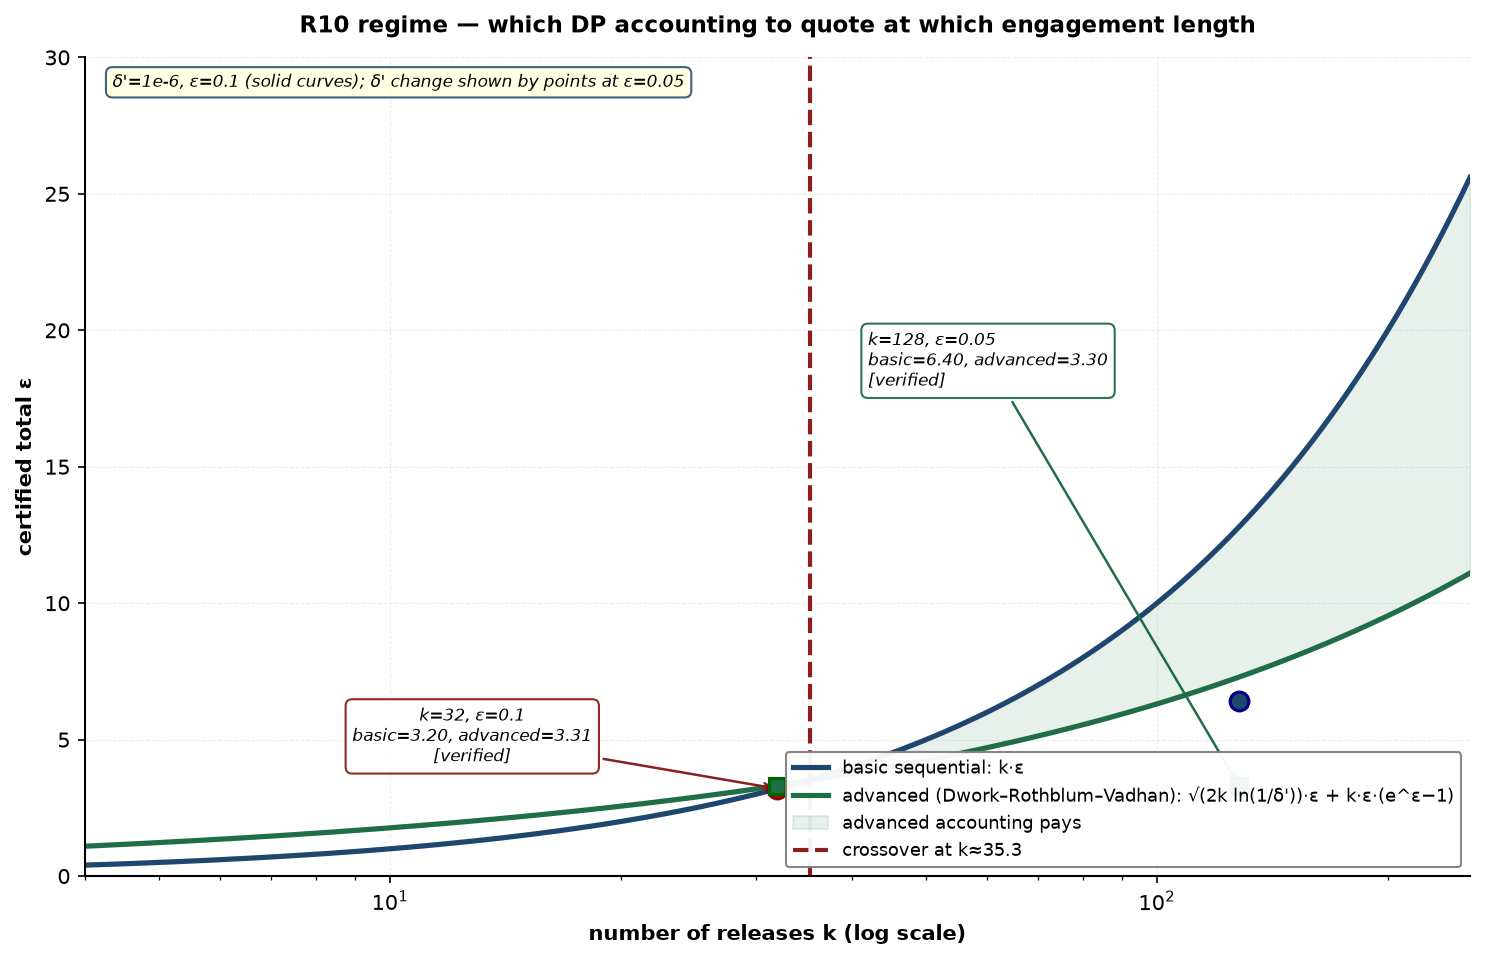
\includegraphics[width=0.88\textwidth]{r10_regime.png}
\caption{Regime diagram for Pillar III: which DP accounting to quote at which engagement length
($\delta'=10^{-6}$). Below the crossover in $k$ the sequential bound $k\varepsilon$ is exact, $\delta$-free, and smaller; past it,
advanced composition's $\sqrt{k}$ scaling wins. The session's two measured points ($k{=}32,\varepsilon{=}0.1$ and
$k{=}128,\varepsilon{=}0.05$) are marked [verified; regenerated by \texttt{a3\_epsilon\_ledger.py}].}
\label{fig:r10reg}
\end{figure}

\textbf{What it buys.} The clean-room contract's budget line becomes an auditable invariant with the same proof shape as the
harbor's bond-conservation result, and the mutation suite shows the invariant has teeth: both canonical atomicity breaks are
caught with shortest traces, and the torn write's deeper crime --- recorded over-spend past the contracted maximum --- is
exhibited concretely.

\begin{boundary}
\textbf{Honest boundary.} Conservation governs \emph{recorded} spend; that all spend is recorded is precisely the
complete-mediation assumption --- Pillar II is the prerequisite, not a nicety. Advanced composition pays only past the
$k$-crossover. And the theorem conserves the meter, not the meaning: choosing per-release $\varepsilon_i$ honestly is the DP
mechanism's obligation, outside this ledger --- differential privacy bounds individual influence in aggregates; it does not
protect the whole dataset, nor Erin's model IP.
\end{boundary}

\section{Pillar IV: canaries with a power curve and a clock}\label{sec:p4}

\onebreath{Independent per-canary misses turn $k$ smuggled canaries into detection probability
$1-\beta^k$; uniform planting turns leak size into a hypergeometric operating curve; and Wald's sequential test against the
permutation null turns leak intensity into an expected time-to-detection --- formal statements in the box below.}

\textbf{Intuition.} Dye packs in bank bundles: each pack fails alone with probability $\beta$, so grabbing $k$ dyed bundles fails
to stain with probability $\beta^k$; how many dyed bundles a thief grabs is set by how much he takes and how densely packs are
planted. The sequential half is quality control: each gate output is a Bernoulli trial, and the sequential probability ratio test
is the optimal stopping rule for ``is this stream leaking?'' Pillars I--III govern what the gate is \emph{allowed} to pass; this
pillar measures what happens when something tries to pass anyway --- ``we have canaries'' is a vibe, and a CISO buys a number.

\begin{thebox}
\textbf{Theorem 4a (power).} With per-canary false-negative rate $\beta$, independent across canaries, a leak carrying $k$ canary
spans is detected with probability $1-\beta^k$. Under uniform planting of $c$ canaries in an $n$-span corpus, a leak of $m$ spans
carries $K\sim\mathrm{Hypergeom}(n,c,m)$ canaries, so $\Pr(\text{detect}\mid m)=1-\mathbb{E}[\beta^K]\approx
1-\bigl(1-\tfrac{c}{n}(1-\beta)\bigr)^m$ --- the operating curve.

\textbf{Theorem 4b (latency, Wald).} Gate outputs are Bernoulli with canary-hit rate $p_0$ under the no-leak permutation null and
$p_1>p_0$ under exfiltration. The SPRT with error targets $(\alpha,b)$ stops, under leak, after expected
$\mathbb{E}_1[N]=\bigl[(1-b)\ln\tfrac{1-b}{\alpha}+b\ln\tfrac{b}{1-\alpha}\bigr]/\mathrm{KL}(p_1\Vert p_0)$ outputs (analogously
$\mathbb{E}_0[N]$ under the null), and is optimal in the Wald--Wolfowitz sense \cite{wald,wald-wolfowitz}.

\textbf{Verification.} $n{=}10^4$, $c{=}100$ (density 1\%), $\beta{=}0.2$: a 100-span leak is caught with probability $0.554$, an
800-span leak at $0.999$; exact hypergeometric, binomial approximation, and simulation agree to Monte-Carlo precision across the
curve, and the $1-\beta^k$ line is confirmed at $k{=}1,2,5$ [internal, \texttt{a4\_canary\_sprt.py}]. SPRT at $p_0{=}10^{-3}$,
$p_1{=}10^{-2}$, $\alpha{=}0.01$, $b{=}0.05$: Wald $\mathbb{E}_1[N]=297$ vs simulated $359$ (the gap is boundary overshoot, which
the Wald identities ignore --- and overshoot only \emph{helps} the error rates: realized miss $0.048\le 0.05$, false alarm
$0.005\le 0.01$); $\mathbb{E}_0[N]=432$ vs simulated $438$. Latency sweep: $10\times$ leak intensity cuts time-to-detection
$\approx 30\times$
[internal].
\end{thebox}

\textbf{Numbers by hand.} At $\beta=0.2$, two smuggled canaries are caught with probability $1-0.04=0.96$ [verified]; the full
operating curve against leak size is Figure~\ref{fig:r11reg}.
\emph{Now you try:} at the same $\beta$, what does a five-canary leak survive with? ($\beta^5=0.00032$ --- detection $0.9997$ [verified].)

\begin{figure}[htbp]
\centering
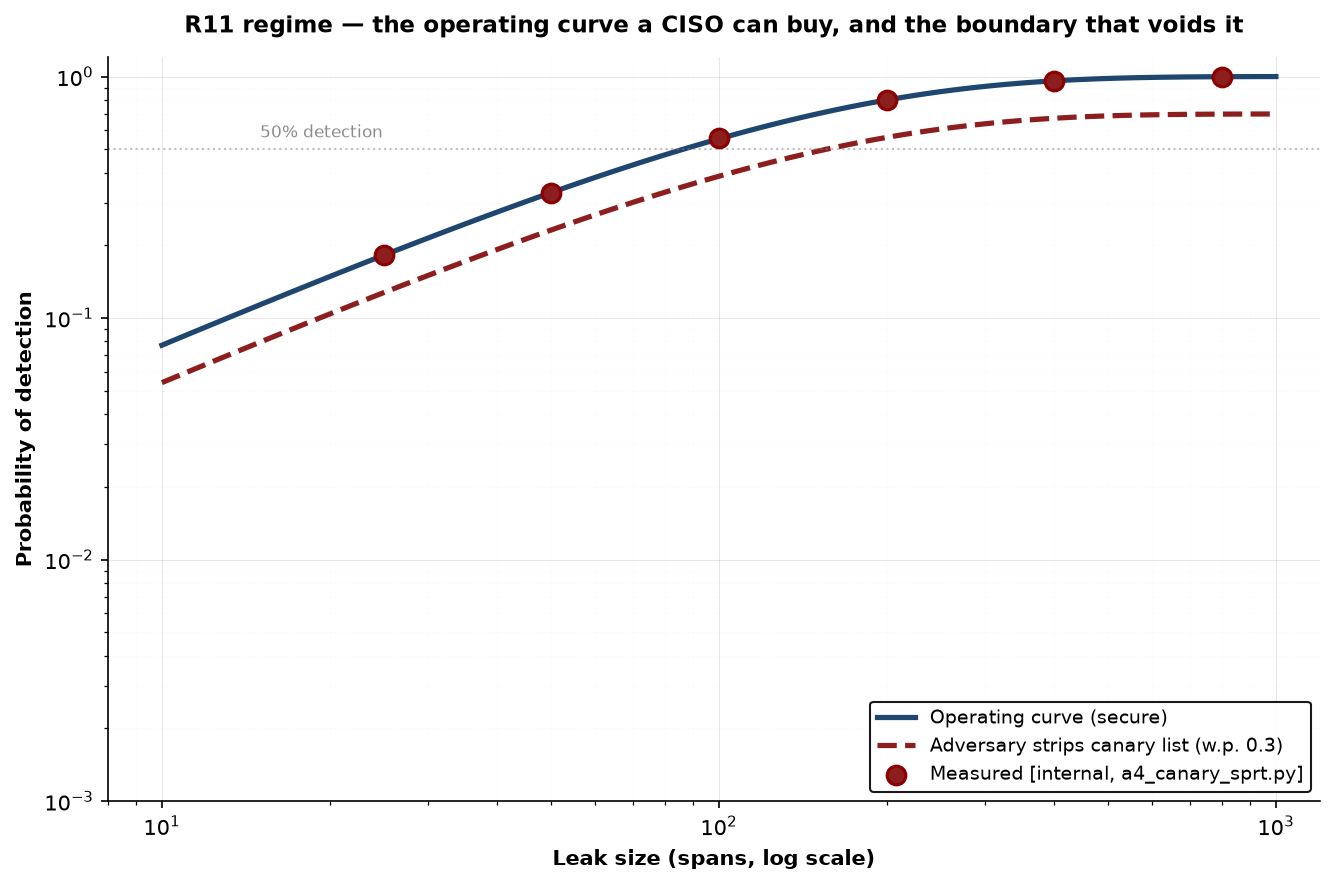
\includegraphics[width=0.92\textwidth]{r11_regime.png}
\caption{Regime diagram for Pillar IV: the operating curve a CISO can buy, and the boundary that
voids it. Left: $\Pr(\text{detect})$ against leak size $m$ at density 1\%, $\beta=0.2$ --- exact, approximate, and simulated agree
[internal, \texttt{a4\_canary\_sprt.py}]. The guarantee's load-bearing regime is secret, uniform planting: an adversary who
obtains the canary list with probability $0.3$ and strips all of them drops measured power from $0.9997$ to $0.698$ at $k{=}5$
[internal].}
\label{fig:r11reg}
\end{figure}

\textbf{What it buys.} The clean-room contract can \emph{quote} $\Pr(\text{detect})=f(\text{leak size})$ and expected alarm
latency per leak intensity --- so the exfiltration bond is re-scoped to its honest job, funding detection and response rather than
pretending to cover unbounded breach damage.

\begin{boundary}
\textbf{Honest boundary.} Independence and \emph{secrecy} of planting are load-bearing: an adversary who obtains the canary list
with probability $0.3$ and strips all of them drops measured power from $0.9997$ to $0.698$ at $k{=}5$ [internal,
\texttt{a4\_canary\_sprt.py}] --- canary secrecy is part of the security boundary, priced explicitly. $\beta$ is a measured
property of the suppressor, not an assumption. The Wald stopping-time formulas are approximations (overshoot inflates
$\mathbb{E}[N]$ ${\sim}20\%$ here, conservatively); and the SPRT detects \emph{statistical} leak signatures --- a single-shot
exfiltration is Theorem 4a's job, not 4b's.
\end{boundary}

\section{The leakage budget: $q\cdot b$ bits, before timing}\label{sec:budget}

The four pillars compose into one information-theoretic account, and the account is deliberately unromantic. If an Erin-visible
channel permits $b$ freely chosen bits per job, a malicious worker can exfiltrate up to $b$ bits through it --- the
noninterference theorem guarantees only that those bits pass through the declared gate, not that they are innocent. Across $q$
jobs the raw capacity is $q\cdot b$ bits; choosing among $s$ timing slots adds up to $\log_2 s$ bits per event, which is why
timing sits outside the possibilistic model and inside \S\ref{sec:cannot}. In Geoffrey Smith's vocabulary \cite{smith-qif}, the
design does not drive min-entropy leakage to zero; it makes leakage a \emph{declared, metered} quantity: fixed schemas, padding,
coarse statuses, query limits, and scheduled release turn an unlimited covert channel into a leakage budget the contract states,
the ledger of Pillar III meters (with DP composition giving the aggregate-feedback portion its formal semantics), and the canaries
of Pillar IV police for evasion around.

The design rule that falls out is quotable: \emph{never negotiate over ``does this output contain a secret'' --- negotiate over
channel capacity.} The first question is undecidable in practice for prose; the second is arithmetic. A contract that grants Erin
a 64-bit status schema per job, 200 jobs, has granted at most $12{,}800$ bits of adversarial capacity before timing --- and can
price, bond, and canary-police exactly that.

\section{What cannot honestly be promised}\label{sec:cannot}

The pitch discipline of this paper is that the boundary list is as prominent as the theorem list. None of the following is
promised, and a contract that implies any of them is overclaiming:

\begin{itemize}
\item \textbf{Zero model leakage with unlimited useful adaptive outputs to Derek.} The
model-confidentiality property is necessarily weaker than the data property, because Derek \emph{intentionally observes}
evaluations of $M$: unlimited adaptive black-box access enables model extraction. Erin's confidentiality is stated relative to the
contracted query-and-output interface, not as absolute secrecy --- the asymmetry is structural, not an engineering gap.
\item \textbf{Zero data leakage with arbitrary natural-language telemetry to Erin.} That channel is
the $q\cdot b$ budget of \S\ref{sec:budget}; ``zero'' is available only at $b=0$.
\item \textbf{Elimination of timing, cache, speculative, firmware, or physical channels.} The
noninterference guarantee is possibilistic; these channels are out of model, declared so, and partially mitigated (padding,
scheduled release) rather than closed.
\item \textbf{Confidentiality through an unapproved external model or tool provider.} A remote API
that reads plaintext is another trusted reader; the model runs inside the confidential domain or the guarantee does not apply.
\item \textbf{Correctness of the answer.} The receipt proves what the measured system reported under
a policy; it does not prove the financial advice was good.
\item \textbf{Literal deletion of information a party already observed}, availability if a key owner
refuses or aborts, or security against colluding hardware vendor, cloud operator, and principal --- each needs a strictly stronger
threat model (MPC/FHE backends are the high-assurance option for narrow fixed computations, not the first implementation for
arbitrary tool-using agents).
\item \textbf{Bounds on minds.} A human who reads a released aggregate may remember it; the system
bounds channels.
\end{itemize}

\section{The lift: from exhaustive model to Isabelle unwinding}\label{sec:lift}

Theorem 1 is exhaustive on a finite model; the general claim over unbounded state is a proof obligation with a known shape.
Rushby's channel-control formulation \cite{rushby} reduces noninterference for a transition system to three local \emph{unwinding
conditions} --- output consistency, step consistency, and local respect --- each a per-transition lemma amenable to mechanization;
the Isabelle Archive of Formal Proofs already carries stateful intransitive-noninterference and noninfluence developments in
exactly this lineage. The finite model of \S\ref{sec:p1} is the blueprint: its local-respect check (Derek-side actions never touch
Erin-observable state) already holds mechanically, its declassification steps are the intransitive ``downgrader'' domain of
Rushby's framework, and the lift consists of restating the clean-room transition relation abstractly and discharging the three
lemmas once, for all depths and all secrets. We flag the lift as the program's stated next obligation for this paper rather than
folding a half-finished mechanization into it; the finite result plus mutation suite is what the lift will certify at scale, not a
substitute for it.

\section{Related work, and what is actually new}\label{sec:related}

\textbf{Imported.} Noninterference and its unwinding proof technique are Goguen--Meseguer
\cite{goguen-meseguer-82,goguen-meseguer-84}; the intransitive/channel-control generalization that models a declassifier as a
distinguished domain is Rushby \cite{rushby}. The enforceability boundary is Ramadge--Wonham supervisory control
\cite{ramadge-wonham} with the Lin--Wonham partial-observation refinement \cite{lin-wonham}. Labels owned by mutually distrustful
principals are the Myers--Liskov decentralized label model \cite{myers-liskov}. Quantitative leakage is Smith's min-entropy
framework \cite{smith-qif}; the composition corollary of Pillar III is Dwork--Rothblum--Vadhan \cite{drv}; the sequential test is
Wald \cite{wald,wald-wolfowitz}; attestation vocabulary is IETF RATS \cite{rats}. Confidential-VM offerings and attested
key-release systems demonstrate the substrate pattern in industry.

\textbf{New, honestly.} No single component theorem above is ours. The contribution is the end-to-end clean-room \emph{design} for
tool-using LLM agents --- dual-attested key release from two mutually distrustful key brokers; whole-worker taint adopted
\emph{because} token-level taint through an LLM is not soundly definable; exactly two declassification gates as the complete exit
set; the $q\cdot b$ leakage-budget contract --- together with the four-pillar assurance argument that makes the design's promise a
theorem schedule rather than a slogan: enforceability (II) says where the boundary can be, noninterference (I) says the boundary
holds, conservation (III) meters what crosses it, and detection (IV) polices evasion with quotable power and latency. The
correction this delivers to practice is the replacement of ``taint analysis prevents exfiltration'' and ``mathematically cannot
phone home'' with the claim that is both stronger and true: \emph{bring the encrypted agent to the encrypted data, and every
release is explicit, gated, and bounded.}

\section*{Reproducibility}

Every [internal] number regenerates from three self-contained Python scripts at seed 20260816, shipped alongside this paper:
\texttt{c1\_noninterference.py} (Pillar I: exhaustive depth-7 check, schedule-independence check, unwinding check, 2/2 mutations
caught with witness traces), \texttt{a3\_epsilon\_ledger.py} (Pillar III: 15-state exhaustive interleaving check, 2000-instance
randomized sweep, 2/2 mutations with shortest crimes, DP composition table), and \texttt{a4\_canary\_sprt.py} (Pillar IV:
$1-\beta^k$ at $k{=}1,2,5$, hypergeometric/binomial/simulated operating curve, SPRT latency and error realization,
canary-stripping boundary experiment). Pillar II's classification table regenerates from \texttt{b3\_controllability.py}. Every
[verified] number is a closed form the reader can recompute from the formulas in the boxes.

\begin{thebibliography}{9}
\bibitem{goguen-meseguer-82} J.~A. Goguen and J.~Meseguer. Security policies and security models. In
\emph{Proc.\ IEEE Symposium on Security and Privacy (Oakland)}, pp.~11--20, 1982.
\bibitem{goguen-meseguer-84} J.~A. Goguen and J.~Meseguer. Unwinding and inference control. In
\emph{Proc.\ IEEE Symposium on Security and Privacy}, 1984.
\bibitem{rushby} J.~Rushby. Noninterference, transitivity, and channel-control security policies.
Technical Report CSL-92-02, SRI International, December 1992.
\bibitem{ramadge-wonham} P.~J. Ramadge and W.~M. Wonham. Supervisory control of a class of discrete
event processes. \emph{SIAM Journal on Control and Optimization}, 25(1):206--230, 1987.
\bibitem{lin-wonham} F.~Lin and W.~M. Wonham. On observability of discrete-event systems.
\emph{Information Sciences}, 44(3):173--198, 1988.
\bibitem{myers-liskov} A.~C. Myers and B.~Liskov. A decentralized model for information flow
control. In \emph{Proc.\ 16th ACM Symposium on Operating Systems Principles (SOSP)}, 1997.
\bibitem{smith-qif} G.~Smith. On the foundations of quantitative information flow. In \emph{Proc.\
FoSSaCS 2009}, LNCS 5504, pp.~288--302, 2009.
\bibitem{drv} C.~Dwork, G.~N. Rothblum, and S.~Vadhan. Boosting and differential privacy. In
\emph{Proc.\ 51st IEEE Symposium on Foundations of Computer Science (FOCS)}, pp.~51--60, 2010.
\bibitem{wald} A.~Wald. Sequential tests of statistical hypotheses. \emph{Annals of Mathematical
Statistics}, 16(2):117--186, 1945.
\bibitem{wald-wolfowitz} A.~Wald and J.~Wolfowitz. Optimum character of the sequential probability
ratio test. \emph{Annals of Mathematical Statistics}, 19(3):326--339, 1948.
\bibitem{rats} H.~Birkholz, D.~Thaler, M.~Richardson, N.~Smith, and W.~Pan. Remote ATtestation
procedureS (RATS) architecture. RFC 9334, IETF, January 2023.
\end{thebibliography}

\end{document}
